\section{Monolayers}
\label{sec:mono}

\subsection{Execution}

The following is conducted for two different unknown TMDCs:
Firstly the scotch tape technique is used, to separate the layers from a thick crystal.
These layers are then transferred to a gel strip, from which they are subsequently transferred onto a silicon wafer that has an SiO$_2$ layer on top.

In order to now find pieces on the wafer that are monolayers, an optical microscope is used, utilizing the fact that due to the different refractive indeces of Si, the SiO$_2$ and the deposited material different thicknesses appear in different colors \cite{benameur2011}.
The samples are then transferred to a widefield microscope, a schematic of which is shown in \cref{fig_widefield}.
%TODO da noch was beschreibendes zu
%TODO numerische Apertur von der Linse
Apart from also having imaging properties, a slit can be inserted into the widefield microscope, to record a spectrum using a basic light spectrometer.
Due to the insertion of the slit, imaging properties in one direction are lost in the process.

\begin{figure}[!ht]
    \centering
    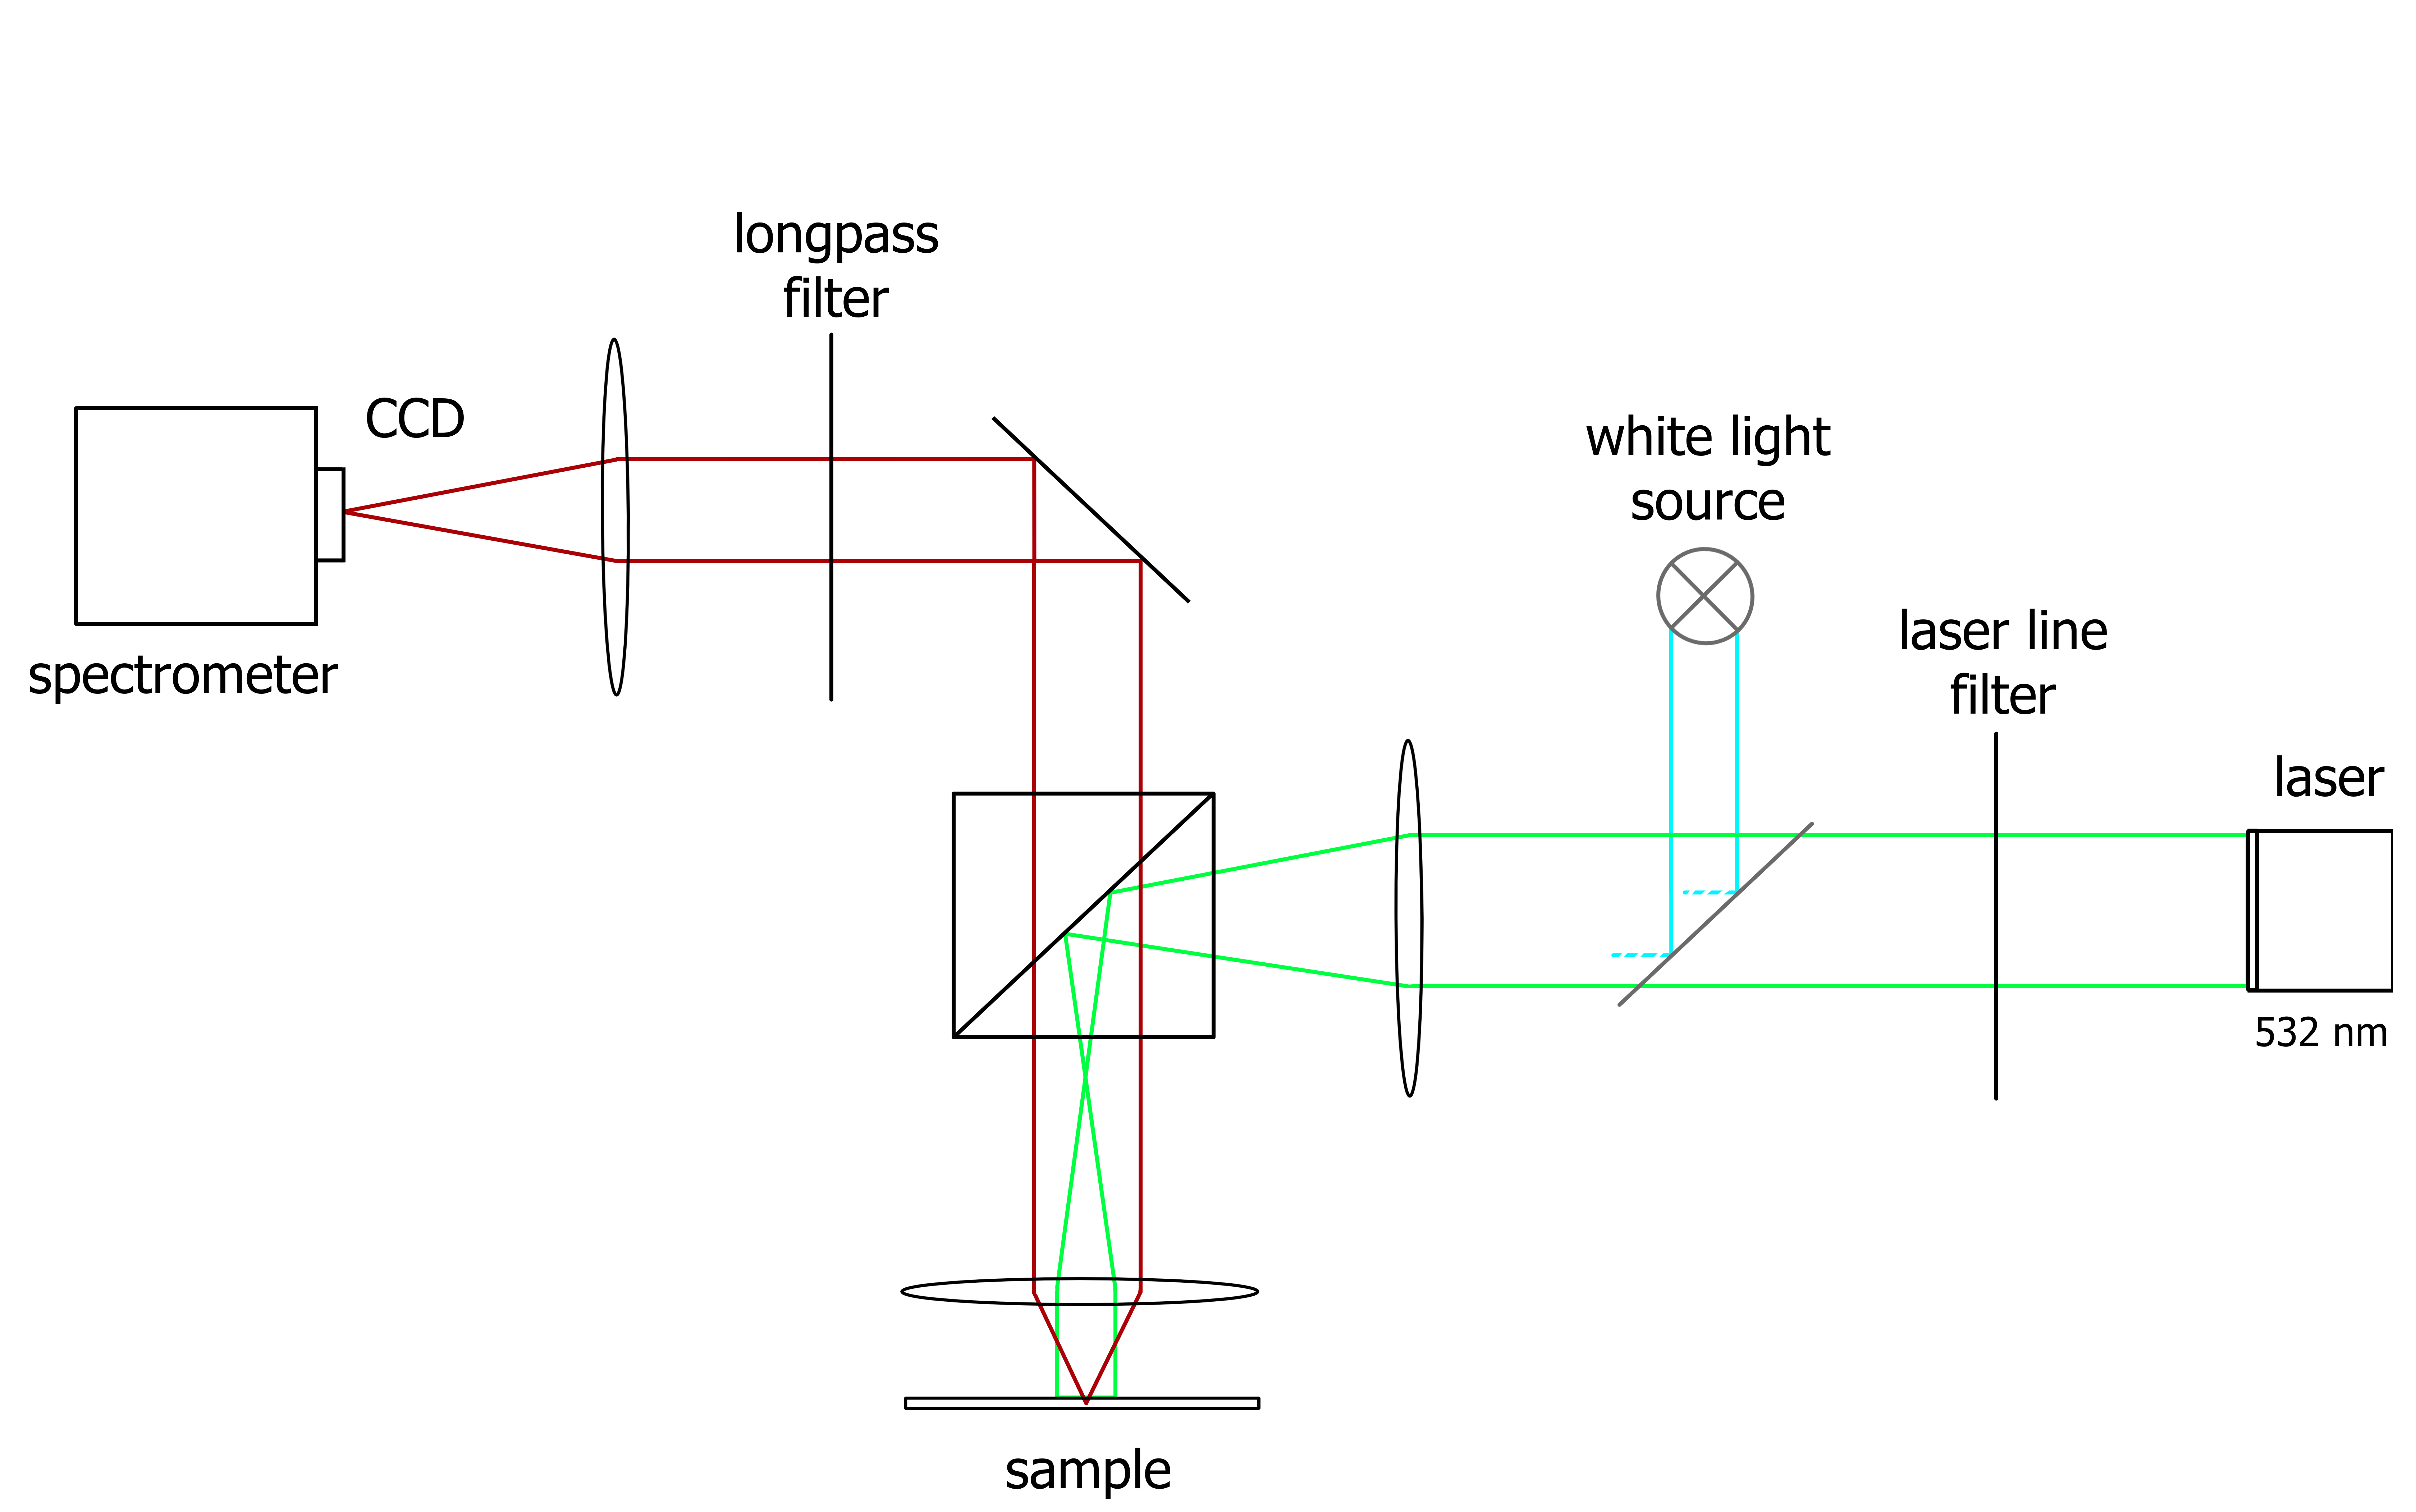
\includegraphics[width=0.7\textwidth]{img/setup1.png}
    \caption{Schematic of the widefield microscope used to record photoluminescence spectra. The detector corresponds to a spectrometer.}
    \label{fig_widefield}
\end{figure}


\subsection{Analysis}
